
\section{Oppgaver}

\subsection{Oppgave A}


\emph{Tegn opp den elektriske kretsen til motoren og lag et diagram av momentene som virker
på motorakslingen.}

\begin{figure}[h]
	\begin{circuitikz}[american]
		\draw
		(0,0) node [anchor = north west] {$u_a+$}
		to [generic=$R_a$] ++ (0,4) 
		to [L=$L_a$] (0,8) node [anchor = north west] {$a$}
		;
		\draw (0,8) to [Telmech=M] ++(3,0) node [anchor = north west] {$b$}
		to (3,0) node [anchor = north west] {$u_a-$}
		;
		        
		\draw 
		(0,12) node [anchor = north west ] {$a1$}
		to (0,10) node [anchor = south west ] {$b1$}
		to [L=Magneter, o-o] (4,10) node [anchor = south east ] {$c1$}
		to (4,12) node [anchor = north east ] {$d1$}
		;
	\end{circuitikz}
	\caption{Skjematiske tegninger}
	\label{fig:el-schematic}
\end{figure}

\begin{figure}[h]
	\centering
	\begin{subfigure}[a]{0.450\textwidth}
		\centering
		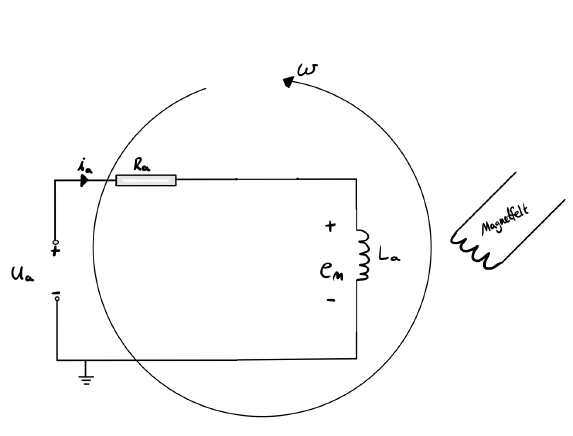
\includegraphics[width = \textwidth]{Images/a_Circuit.png}
		\caption{}{Kretsskjema som samsvarer med Figur \ref{fig:el-schematic}}
		
	\end{subfigure}
	\begin{subfigure}[a]{0.450\textwidth}
		\centering
		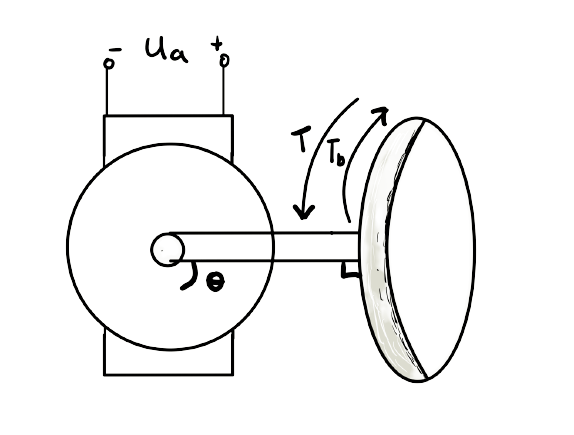
\includegraphics[width = \textwidth]{Images/a_Motor.png}
		\caption{}{Motorens aksling og kreftene som virker på akslingen}
		\label{fig:el-drawing-hand}
	\end{subfigure}
	\caption{Skjematisk tegning av motorens oppbygning}
	\label{fig:schematics}
\end{figure}

Den elektriske kretsen viser et anker mellom a og b med intern spole-$L_a$ og en intern motstand-$R_a$.
De eksterne magnetene fra a1 til d1 vil kunne skyve og trekke motoren avhengig av hvilken strømretning som er i ankeret. Strømretningen bytter for hver enhet av en gitt vinkel. Ankeret roterer fordi spenningskontaktene bytter plass i kretsen i $u_a+$ og $u_a-$.


\subsection{Oppgave B}

\emph{Bruk symbolene ovenfor og vis hvordan du setter opp de to differensiallikningene som
	beskriver den elektriske og den mekaniske delen i likestrømmotoren.}\\

For den elektriske kretsen bruker vi Kirchoff´s spenningslov med formler for spenning:\\
\begin{tabular}{ll}
	Tilført spenning:                   & $u_a$                       \\
	Spenning over motstand:             & $u_R(t) = R\cdot i_R$       \\
	Spenning over spole:                & $u_L(t) = L\frac{di_L}{dt}$ \\
	Indusert spenning fra magnetfeltet: & $e_m$                       
\end{tabular}\\

Disse gir oss følgende likning: 
\begin{align}
	u_a & = Ri_a + L\frac{di_a}{dt} + e_m &   
	\label{eqn:ode_elec}
\end{align}

Momentene som virker på ankeret er:

\begin{tabular}{ll}
	Motormoment:                             & $T = K_t\cdot i_a$       \\
	Friksjon:                                & $T_b = b\cdot \omega$    \\
	Dreiemoment ved konstant treghetsmoment: & $\tau = J_m\cdot \alpha$ 
\end{tabular}

Dette gir oss likningen:
\begin{align*}
	\tau & = T - T_b &   \\
	J_m\alpha &=  K_ti_a - b\omega
\end{align*}
Og kan videre omskrives som:
\begin{align}
	J_m\alpha + b\omega & = K_ti_a\nonumber &   \\
	J_m\frac{d^2\theta}{dt^2} + b\frac{d\theta}{dt} &= K_ti_a\nonumber\\
	\frac{d^2\theta}{dt^2} + \frac{b}{J_m}\frac{d\theta}{dt} &= \frac{K_ti_a}{J_m}
	\label{eqn:ode_mech}
\end{align}\\


\subsection{Oppgave C}

\emph{Sett inn tallverdiene og vis at likningene er gitt ved:\\ $\frac{di_a}{dt} + 10i_a + \omega = u_a$,  $ \frac{d^2\theta}{dt^2} + 0.1\frac{d\theta}{dt} = 100i_a$}\\
   

Setter vi inn tallverdiene fra tabellen gir dette oss følgende likninger;\\
Elektrisk \eqref{eqn:ode_elec}:
\begin{align*}
	R_a\cdot i_a + L_a\cdot \frac{di_a}{dt} + K_e\cdot \omega & = u_a &   \\
	10\cdot i_a + 1\cdot \frac{di_a}{dt} + K_e\cdot \omega    & = u_a &   \\
	1\cdot \frac{di_a}{dt} + 10i_a + 1\cdot \omega &= u_a \\
	\frac{di_a}{dt} + 10i_a + \omega &= u_a\\
\end{align*}\\
Mekanisk \eqref{eqn:ode_mech}:
\begin{align*}
	\frac{d^2\theta}{dt^2} + \frac{b}{J_m}\frac{d\theta}{dt}             & = \frac{K_ti_a}{J_m}        \\
	\frac{d^2\theta}{dt^2} + \frac{0.001}{0.01} \cdot \frac{d\theta}{dt} & = \frac{K_t\cdot i_a}{0.01} \\
	\frac{d^2\theta}{dt^2} + 0.1\frac{d\theta}{dt}                       & = 1\cdot i_a\cdot 100       \\
	\frac{d^2\theta}{dt^2} + 0.1\dfrac{d\theta}{dt}                      & = 100i_a                    
\end{align*}
    
\subsection{Oppgave D}

\emph{Velg tilstandene $x_1 = 1$, og $x_2 = \theta$ og $x_3 = \omega$. Still opp tilstandsrommodellen for motoren med ankerspenningen som pådrag, $u = u_a$, og motorvinkelen som måling, $y = \theta$.}
    
Tilstandsvariabler:

\begin{align*}
	x_1 & = i_a    \\        
	x_2 & = \theta \\     
	x_3 & = \omega \\     
	u   & = u_a    \\       
	y   & = \theta 
\end{align*}
   
Systemet uttrykt med tilstandsvariablene:
   
\begin{align*}
	\dot x_1 & = \frac{di_a}{dt} = -10i_a - \omega + u_a                 \\
	         & = -10x_1 - x_3 + u                                        \\
	\dot x_2 & = \frac{d\theta}{dt} = \omega                             \\
	         & = x_3                                                     \\
	\dot x_3 & = \frac{d^2\theta}{dt^2} = 100i_a - 0.1\frac{d\theta}{dt} \\
	         & = 100x_1 - 0.1x_3                                         \\
	y        & = x_2                                                     \\
\end{align*}

Tilstandsrommodellen i formen $ \dot{\vec{x}} = A\vec{x} + Bu $, $ \vec{y} = C\vec{x} + Du $. I vårt tilfelle er D = 0.

\begin{equation}
	\begin{aligned}
		\dot{\vec{x}} &=
		\begin{bmatrix}
		-10 & 0 & -1   \\
		0   & 0 & 1    \\
		100 & 0 & -0.1 \\
		\end{bmatrix}
		\Vec{x}
		+
		\begin{bmatrix}
		1\\
		0\\
		0\\
		\end{bmatrix}
		u\\
		\vec{y} &= 
		\begin{bmatrix}
		0   & 1 & 0    \\
		\end{bmatrix}
		\Vec{x}
		\label{ss-model}
	\end{aligned}
\end{equation}
    
\subsection{Oppgave E}

\emph{Bestem egenverdiene til systemet. Hvor stor er egenfrekvensen og den relative
dempningen til motoren?}

Egenverdier:
\begin{equation*}
	\begin{aligned}
		(\dot{\vec{x}} - \lambda I) &=
		\begin{bmatrix}
		-10-\lambda & 0        & -1           \\
		0           & -\lambda & 1            \\
		100         & 0        & -0.1-\lambda \\
		\end{bmatrix}\\\\
		det(\dot{\vec{x}} - \lambda I) &= -\lambda ^3 -10,1\lambda ^2 - 101\lambda = 0\\\\
		\lambda _1 &= 0\\\\
		\lambda _2 &= \frac{1}{20} (-101-i\sqrt{30199})\\\\
		\lambda _3 &= \frac{1}{20} (-101 + i\sqrt{30199})\\\\
	\end{aligned}
\end{equation*}
Vi bruker at egenverdiene til et system = polene til transferfunksjonene ($\lambda = s$) og finner:
Relativ dempingsrate:
\begin{equation}
	\begin{aligned}
		s & = -\sigma \pm i\omega \implies \sigma & = \frac{101}{20} & \approx 5.05 
	\end{aligned}
	\label{damping-rate}
\end{equation}
Egenfrekvens:
\begin{equation}
	\begin{aligned}
		s & = -\sigma \pm i\omega \implies \omega & = \frac{\sqrt{30199}}{20} & \approx 8.69 
	\end{aligned}
	\label{natural-freq}
\end{equation}

\subsection{Oppgave F}
    
\emph{Bruk Laplace-transformasjon og finn transferfunksjonen til motoren, $H(s) = \frac{\theta(s)}{U_a(s)}$}
\begin{center}
	\begin{tabular}{ll}
		$u_a = \frac{di_a}{dt} + Li_a + \omega$               & $100i_a{} = \frac{d^2\theta}{dt^2} + 0.1\frac{d\theta}{dt}$ \\
		$u_a = \frac{di_a}{dt} + 10i_a + \frac {d\theta}{dt}$ & $U_a = I_a s + 10I_a + \theta s$                            \\
		$U_a = I_a s + 10I_a + \theta s$                      & $100I_a = (0.1s + s^2) \theta$                              \\
		$I_a = \frac {U_a - \theta s} {s+10}$                 & $\theta = \frac {100I_a}{s(s+0.1)}$                         \\
		        
	\end{tabular}
\end{center}
Setter inn $I_a$ i uttrykket til $\theta$:

\begin{align*}
	\theta                             & = \frac{100 \cdot \frac{U_a-\theta s}{s+10}}{s(s+0.1)} \\
	\theta                             & = \frac{100U_a - 100\theta s}{s(s+0.1)(s+10)}          \\
	\theta s(s+0.1)(s+10)              & = 100 U_a - 100 \theta s                               \\
	\theta (s(s+0.1)(s+10) + 100s)     & = 100 U_a                                              \\
	H (s) = \frac{\theta (s)}{U_a (s)} & = \frac{100}{s^3+10.1 s^2 + 101s}                      
\end{align*}


\subsection{Oppgave G}

\emph{Lag et MATLAB-script hvor du legger inn tilstandsrom-modellen for dette systemet.
	Bestem også transfer-funksjonen til systemet ved hjelp av Matlab. Bestem
	sprangresponsen til motoren. Gi en tolkning av responsen gitt ved karakteristiske
størrelser i responsen. Er systemet stabilt?}

Uten tilbakekobling, og med konstant påtrykt spenning på ankeret, vil motoren bare gå og gå. Altså vil den målte vinkelen bare øke og øke, tilnærmet lik $\theta = \omega t$. Systemet, hvor målet er å stabilisere ankeret på en gitt vinkel, er derfor ustabilt. Figur \ref{fig:step_unstable} viser sprangresponsen til systemet uten tilbakekobling. For å finne overføringsfunksjonen brukes Matlab-funksjonen ss2tf, som returner følgende:
$$G(s) = \frac{100}{s^3 + 10.1s^2 + 101s} $$

\begin{figure}[h]
	\centering
	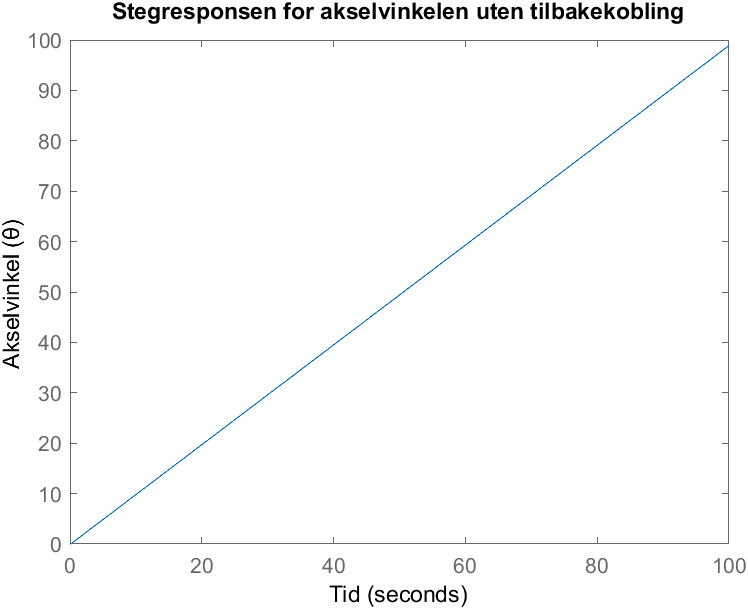
\includegraphics[width=100mm]{Images/g_StepResponse.png}
	\caption{Matlab-plot av sprangresponsen til akselvinkelen uten tilbakekobling}
	\label{fig:step_unstable}
\end{figure}


\subsection{Oppgave H}

\emph{Vi måler motorvinkelen og lager en tilbakekopling til pådraget. Velg en proporsjonalregulator med forsterkning $K_p = 1$. Lag en lukket sløyfe i Matlab og test systemet med et sprang i referansen. Vil motoren klare å stille seg inn på en gitt vinkelreferanse uten stasjonært avvik? Begrunn svaret. Gi en tolkning av responsen gitt ved karakteristiske størrelser}

En ren proporsjonalregulator med forsterkning lik 1 tilsvarer en direkte kobling mellom avviket og systemets overføringsfunksjon.
Ja, motoren vil klare å stille seg inn på ønsket vinkel, av to grunner. Først og fremst er det lav forsterkning på regulatoren, det medfører at det ikke oppstår økende oscillasjoner i systemet. \\Med en P-regulator er det vanlig og få et stasjonæravvik. Når avviket er null og akselen er i riktig vinkel, vil pådraget være 0. Siden det ikke er noen krefter som vil prøve å dytte motoren i noen retning når pådraget er 0, vil det ikke oppstå noe stasjonært avvik i dette tilfelle. \\\\Hvis vi derimot har en konstant endring i ønsket vinkel, for eksempel en sinuskurve, ser vi at målt vinkel alltid henger litt etter. Ved stadig endring av referanse vil vi alltid ha et varierende avvik så lenge vi kun bruker P-regulator. I det tilfelle ville det vært gunstig å legge på D-ledd og muligens I-ledd.
    
Vi kan også se på det matematisk. Siden alle polene har negativ realverdi vet vi at systemet er stabilt og kan bruke følgende:
$$e_{stasjonæravvik} = \lim_{t \to \infty} e(t) = \lim_{s \to 0} sE(s) $$
For sprangrespons, $U(s) = \frac{1}{s}$:
\begin{align*}
	E(s) = \frac{U(s)}{1+H_R(S)G(S)} & = \frac{\frac{1}{s}}{1 + 1\cdot\frac{100}{s^3 + 10.1s^2 + 101s}}                                 \\
	E(s)                             & = \frac{1}{s} \cdot \frac{s^3 + 10.1s^2 + 101s}{s^3 + 10.1s^2 + 101s + 100}                      \\
	\lim_{s \to 0} sE(s)             & = \lim_{s \to 0} s\cdot\frac{1}{s} \cdot \frac{s^3 + 10.1s^2 + 101s}{s^3 + 10.1s^2 + 101s + 100} \\
	e_{stasjonæravvik}              & = \frac{0}{100} = 0                                                                              
\end{align*}
    
I figur \ref{fig:step_stable_char} sees karakteristikken til sprangresponen, hentet fra MatLab. \\
\begin{tabular}{r l}
	Stigningstid:  & 1.96s \\
	Overskridelse: & 0\%   \\
	Innstillingstid:  & 3.66s 
\end{tabular}
\label{itm:steady-state}

\begin{figure}[h]
	\centering
	\begin{subfigure}[a]{0.450\textwidth}
		\centering
		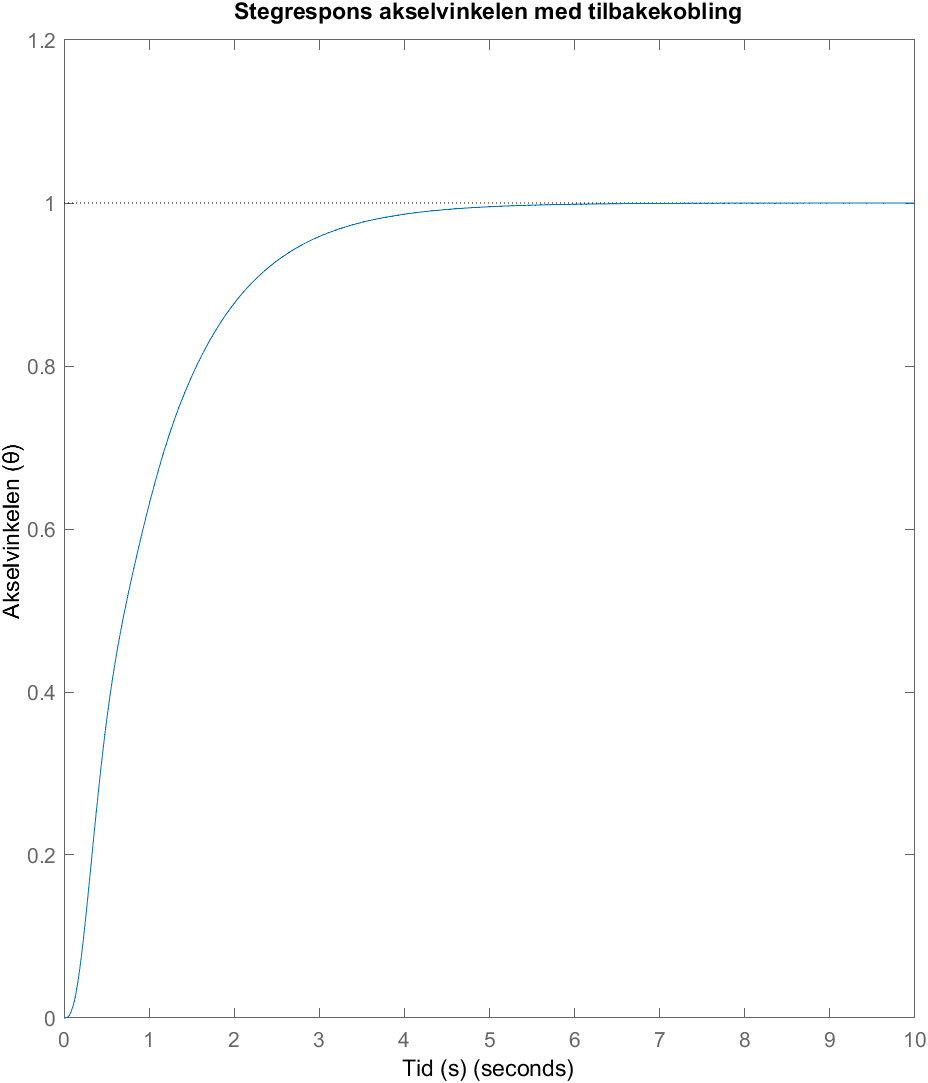
\includegraphics[width = \textwidth]{Images/h_StepResponse.png}
		\caption{}{Sprangrespons}
	\end{subfigure}
	\begin{subfigure}[a]{0.450\textwidth}
		\centering
		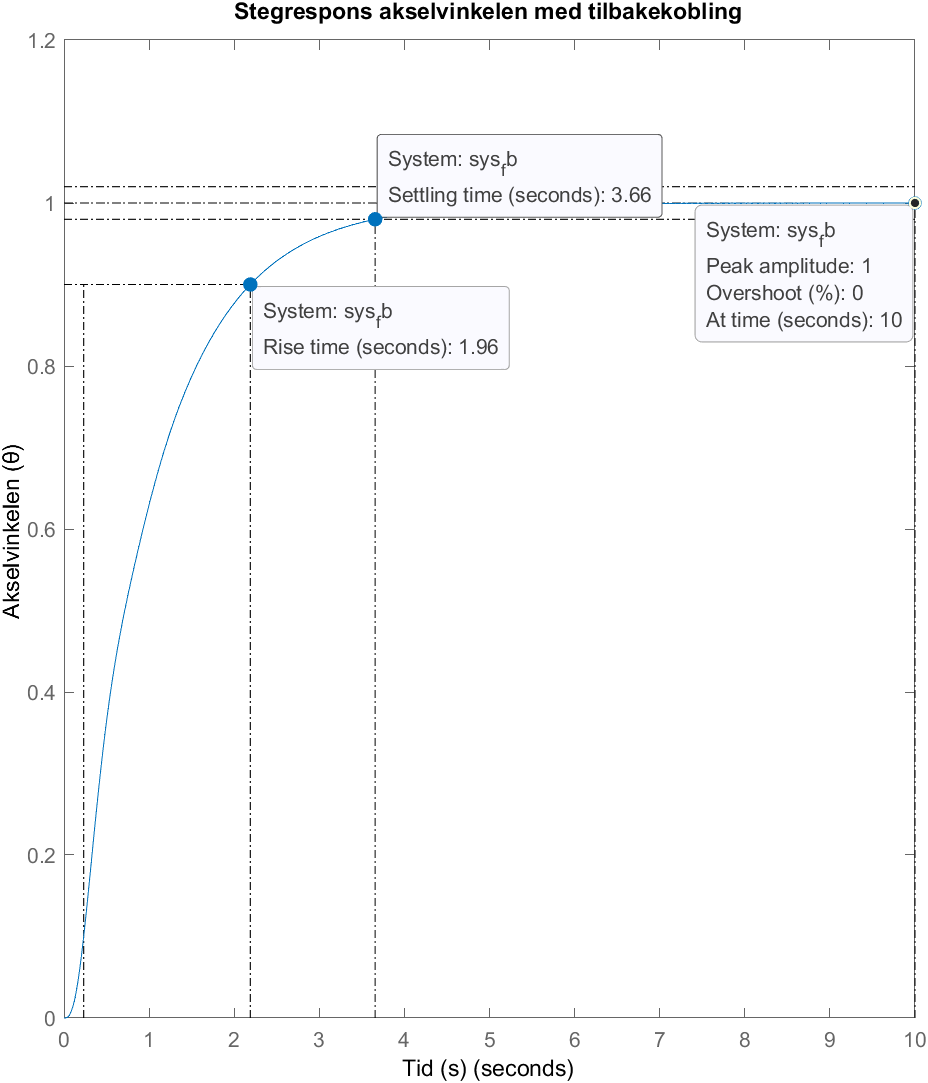
\includegraphics[width = \textwidth]{Images/h_StepResponseCharacterisics.png}
		\caption{}{Karakteristikk for sprangresponsen}
		\label{fig:step_stable_char}
	\end{subfigure}
	\caption{Matlab-plot av sprangresponsen til akselvinkelen med tilbakekobling}
	\label{fig:step_stable}
\end{figure}

\subsection{Oppgave I}

\emph{Prøv ut reguleringen med ulike forsterkninger $K_p$ for regulatoren. Hvordan påvirkes
	responsen til systemet når forsterkningen endres? Hva skjer dersom $K_p$ er veldig høy?}\\

Lavere forsterkning $K_p$ medfører bare at systemet bruket betydelig lengre tid på nå stabilt. 
Mer og mer forsterkning gjør systemet mindre stabilt. Allerede ved $K_p = 2$ kan vi se en mindre jevn kurve på vinkelen. Med $K_p = 11$ slutter systemet og stabilisere seg på en verdi og oscillasjonene øker.

\subsection{Oppgave J}

\emph{Bestem transferfunksjonen til reguleringssløyfen, altså følgeforholdet $M(s)$, med manuell regning. Vis ved beregning hvordan systemet følger et sprang og en rampe i referansen.}

\begin{align*}
	M(s)                           & = \frac{Y(s)}{U(s)}                                       \\
	(U(s) - Y(s)) \cdot H_R(s)G(s) & = Y(s), \quad H_R(s) = 1                                  \\
	Y(s)(1 + G(s))                 & = U(s)G(s)                                                \\
	M(s) = \frac{Y(s)}{U(s)}       & = \frac{G(s)}{1 + G(s)}                                   \\
	M(s)                           & = \frac{s^3 + 10.1s^2 + 101s}{s^3 + 10.1s^2 + 101s + 100} \\\\
	M(s) = \frac{Y(s)}{U(s)}       & \implies Y(s) = U(s)M(s)                                  \\
\end{align*}
Sprangrespons, $U(s) = \frac{1}{s}$:
\begin{align*}
	Y(s) & = U(s)\cdot M(s)                                                          \\
	Y(s) & = \frac{1}{s}\cdot\frac{s^3 + 10.1s^2 + 101s}{s^3 + 10.1s^2 + 101s + 100} \\
	Y(s) & = \frac{s^2 + 10.1s + 101}{s^3 + 10.1s^2 + 101s + 100}                    
\end{align*}
Ramperespons, $U(s) = \frac{1}{s^2}$:
\begin{align*}
	Y(s) & = U(s)\cdot M(s)                                                            \\
	Y(s) & = \frac{1}{s^2}\cdot\frac{s^3 + 10.1s^2 + 101s}{s^3 + 10.1s^2 + 101s + 100} \\
	Y(s) & = \frac{s^2 + 10.1s + 101}{s^4 + 10.1s^3 + 101s^2 + 100s}                   
\end{align*}